\subsubsection*{\large Используемые структуры}
\begin{lstlisting}[caption=Структура \_IO\_FILE]
struct _IO_FILE {
	int _flags;           /* High-order word is _IO_MAGIC; rest is flags. */
	#define _IO_file_flags _flags
	/* The following pointers correspond to the C++ streambuf protocol. */
	/* Note:  Tk uses the _IO_read_ptr and _IO_read_end fields directly. */
	char* _IO_read_ptr;   /* Current read pointer */
	char* _IO_read_end;   /* End of get area. */
	char* _IO_read_base;  /* Start of putback+get area. */
	char* _IO_write_base; /* Start of put area. */
	char* _IO_write_ptr;  /* Current put pointer. */
	char* _IO_write_end;  /* End of put area. */
	char* _IO_buf_base;   /* Start of reserve area. */
	char* _IO_buf_end;    /* End of reserve area. */
	/* The following fields are used to support backing up and undo. */
	char *_IO_save_base; /* Pointer to start of non-current get area. */
	char *_IO_backup_base;  /* Pointer to first valid character of backup area */
	char *_IO_save_end; /* Pointer to end of non-current get area. */
	struct _IO_marker *_markers;
	struct _IO_FILE *_chain;
	int _fileno;
	#if 0
	int _blksize;
	#else
	int _flags2;
	#endif
	_IO_off_t _old_offset; /* This used to be _offset but it's too small.  */
	#define __HAVE_COLUMN /* temporary */
	/* 1+column number of pbase(); 0 is unknown. */
	unsigned short _cur_column;
	signed char _vtable_offset;
	char _shortbuf[1];
	/*  char* _save_gptr;  char* _save_egptr; */
	_IO_lock_t *_lock;
	#ifdef _IO_USE_OLD_IO_FILE
};
\end{lstlisting}

%\begin{lstlisting}[caption=Структура filename]
%	struct stat {
%		dev_t     st_dev;         /* ID устройства с файлом */
%		ino_t     st_ino;         /* номер inode */
%		mode_t    st_mode;        /* права доступа */
%		nlink_t   st_nlink;       /* кол-во жёстких ссылок */
%		uid_t     st_uid;         /* ID пользователя-владельца */
%		gid_t     st_gid;         /* ID группы-владельца */
%		dev_t     st_rdev;        /* ID устройства (если это спец. файл) */
%		off_t     st_size;        /* полный размер в байтах */
%		blksize_t st_blksize;     /* размер блока ввода-вывода
%		файловой системы */
%		blkcnt_t  st_blocks;      /* кол-во выделенных блоков по 512Б */
%		/* Начиная с Linux 2.6, ядро поддерживает точность до
%		наносекунд в следующих полям меток времени.
%		Подробней о версиях до Linux 2.6, смотрите ЗАМЕЧАНИЯ. */
%		struct timespec st_atim;  /* время последнего доступа */
%		struct timespec st_mtim;  /* время последнего изменения */
%		struct timespec st_ctim;  /* время последней смены состояния */
%		#define st_atime st_atim.tv_sec      /* для обратной совместимости */
%		#define st_mtime st_mtim.tv_sec
%		#define st_ctime st_ctim.tv_sec
%	};
%\end{lstlisting}

\pagebreak

\begin{lstlisting}[caption=Структура filename]
struct stat {
	dev_t     st_dev;         /* device */
	ino_t     st_ino;         /* inode */
	mode_t    st_mode;        /* access rules */
	nlink_t   st_nlink;       /* links */
	uid_t     st_uid;         /* UID*/
	gid_t     st_gid;         /* GID*/
	dev_t     st_rdev;        /* ID device (special file) */
	off_t     st_size;        /* byte size */
	blksize_t st_blksize;     /* size of system IO block */
	blkcnt_t  st_blocks;      /* count of allocated blocks per 512 bytes */
	struct timespec st_atim;  /* last launch */
	struct timespec st_mtim;  /* last update */
	struct timespec st_ctim;  /* last change */
	#define st_atime st_atim.tv_sec      /* backward compatibility */
	#define st_mtime st_mtim.tv_sec
	#define st_ctime st_ctim.tv_sec
};
\end{lstlisting}


\section*{Программа 1}

В данной программе создаётся 1 дескриптор файла и на его основе создаются 2 объекта структуры struct \_IO\_FILE.
Устанавливается буфер размером 20 байт и происходит поочерёдное обращение к каждой структуре для чтения одного символа из файла и вывода его на экран. Чтение продолжается пока есть возможность читать, обращаясь хотя бы к одной из структур.

\subsection*{Однопоточный вариант}

\begin{lstlisting}[caption=Однопоточный вариант]
#include <stdio.h>
#include <fcntl.h>

int main()
{
	int fd = open("alphabet.txt",O_RDONLY);
	FILE *fs1 = fdopen(fd,"r");
	char buff1[20];
	setvbuf(fs1,buff1,_IOFBF,20); // full buffering
	FILE *fs2 = fdopen(fd,"r");
	char buff2[20];
	setvbuf(fs2,buff2,_IOFBF,20); // full buffering\\
\end{lstlisting}
\begin{lstlisting}[caption=Однопоточный вариант]
	int flag1 = 1, flag2 = 1;
	while(flag1 == 1 || flag2 == 1)
	{
		char c;
		flag1 = fscanf(fs1,"%c",&c);
		if (flag1 == 1) 
		{
			fprintf(stdout,"%c",c);
		}
		flag2 = fscanf(fs2,"%c",&c);
		if (flag2 == 1) 
		{ 
			fprintf(stdout,"%c",c); 
		}
	}
	return 0;
}
\end{lstlisting}

Результат работы однопоточного варианта представлен на рисунке \ref{p1_one}.

\begin{figure}[ht!]
	\centering
	
\includegraphics[scale=1]{p1_one}
	\caption{Результат работы однопоточной программы}
	\label{p1_one}
\end{figure}

\subsection*{Многопоточный вариант}

\begin{lstlisting}[caption=Многопоточный вариант]
#include <stdio.h>
#include <fcntl.h>
#include <pthread.h>

void *thread(void *args)
{
	int fd = *(int *) args;
	FILE *fs = fdopen(fd,"r");
	char buff[20];
	setvbuf(fs,buff,_IOFBF,20); // full buffering
	int flag = 1;
	while(flag == 1)
	{
		char c;
		flag = fscanf(fs,"%c",&c);
\end{lstlisting}		
\begin{lstlisting}[caption=Многопоточный вариант]
		if (flag == 1) 
		{
			fprintf(stdout,"%c",c);
		}
	}
}

int main()
{
	int fd = open("alphabet.txt",O_RDONLY);
	pthread_t th1;
	pthread_t th2;
	pthread_create(&th1, NULL, thread, &fd);
	pthread_create(&th2, NULL, thread, &fd);
	pthread_join(th1, NULL);
	pthread_join(th2, NULL);
	return 0;
}
\end{lstlisting}

Результат работы многопоточного варианта представлен на рисунке \ref{p1_two}.

\begin{figure}[ht!]
	\centering
	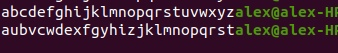
\includegraphics[scale=1]{p1_two}
	\caption{Результат работы многопоточной программы}
	\label{p1_two}
\end{figure}

\section*{Анализ результата}

При первом вызове функции fscanf буфер затронутого экземпляра структуры \_IO\_FILE полностью заполняется 20 символами (от a до t), а значит файловый указатель перемещается на 20 символов вправо. Второй вызов fscanf с другим экземпляром структуры \_IO\_FILE также заполняет его буфер максимальным оставшимся количеством символов (от t до z) и перемещает файловый указатель в конец файла. Дальнейшие вызовы никак не меняют состояние буферов, так как данные из файла уже считаны. При вызове fprintf буквы из каждого буфера поочерёдно выводятся на экран. Таким образом, полученный результат связан исключительно с буферизацией ввода.

\begin{figure}[ht!]
	\centering
	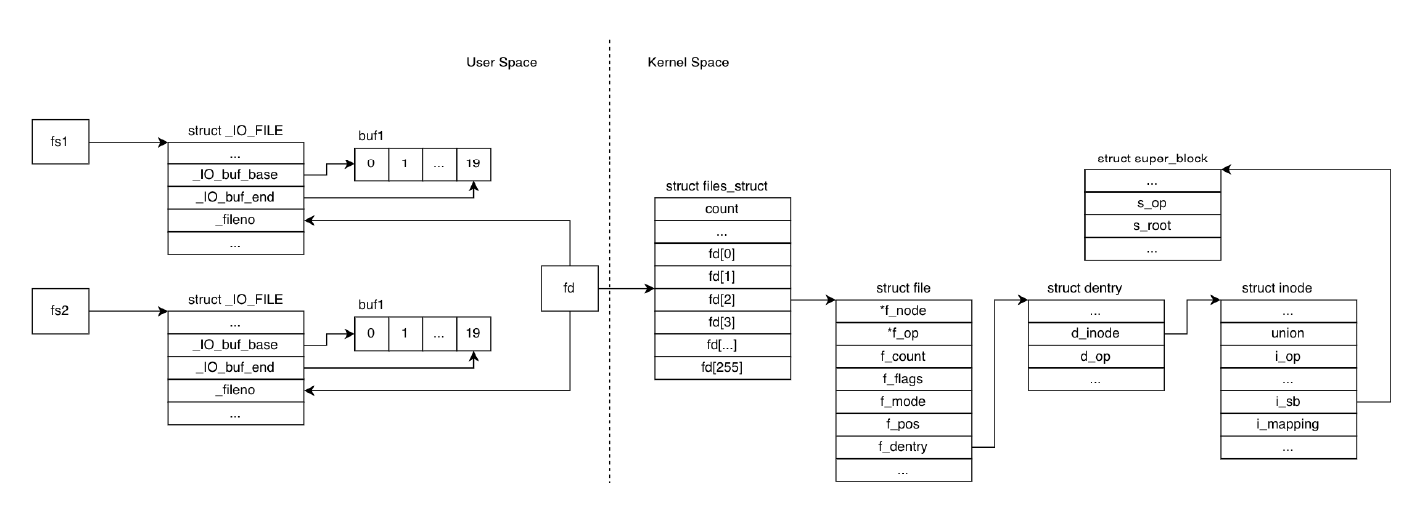
\includegraphics[scale=0.45]{p1_schema}
	\caption{Схема связи структур}
\end{figure}


\section*{Программа 2}

В данной программе создаётся два дескриптора одного файла.
Далее происходит поочерёдное обращение к каждому дескриптору для чтения одного символа из файла и вывода одного символа на экран. Чтение продолжается пока есть возможность читать, обращаясь к каждому дескриптору.

\subsection*{Однопоточный вариант}

\begin{lstlisting}[caption=Однопоточный вариант]
#include <unistd.h>
#include <fcntl.h>

int main()
{
	char c;    
	int fd1 = open("alphabet.txt",O_RDONLY);
	int fd2 = open("alphabet.txt",O_RDONLY);
	int flag = 1;
	while(flag == 1)
	{
		if ((flag = read(fd1,&c,1)) == 1)
			write(1,&c,1);
		if (flag == 1 && (flag = read(fd2,&c,1)) == 1)
			write(1,&c,1);
	}
	close(fd1);
	close(fd2);
	return 0;
}
\end{lstlisting}

Результат работы однопоточного варианта представлен на рисунке \ref{p2_one}.

\begin{figure}[ht!]
	\centering
	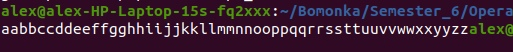
\includegraphics[scale=0.8]{p2_one}
	\caption{Результат работы однопоточной программы}
	\label{p2_one}
\end{figure}

\subsection*{Многопоточный вариант}

\begin{lstlisting}[caption=Многопоточный вариант]
#include <unistd.h>
#include <fcntl.h>
#include <pthread.h>

void *thread(void *args)
{
	char c;
	int fd = open("alphabet.txt",O_RDONLY);
	int flag = 1;
	while (flag == 1)
	{
		if ((flag = read(fd, &c, 1)) == 1)
		write(1, &c, 1);
	}
	close(fd);
	return NULL;
}

int main()
{
	pthread_t th1;
	pthread_t th2;
	pthread_create(&th1, NULL, thread, NULL);
	pthread_create(&th2, NULL, thread, NULL);
	pthread_join(th1, NULL);
	pthread_join(th2, NULL);
	return 0;
}
\end{lstlisting}

Результат работы многопоточного варианта представлен на рисунке \ref{p2_two}.

\begin{figure}[ht!]
	\centering
	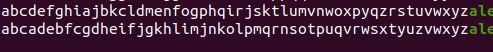
\includegraphics[scale=1]{p2_two}
	\caption{Результат работы многопоточной программы}
	\label{p2_two}
\end{figure}

\section*{Анализ результата}

Чтение символа из файла для каждого дескриптора происходит независимо от другого, для каждого дескриптора существует файловый указатель, поэтому в результате получается удвоение каждого символа. Таким образом файл читается полностью 2 раза.

\begin{figure}[ht!]
	\centering
	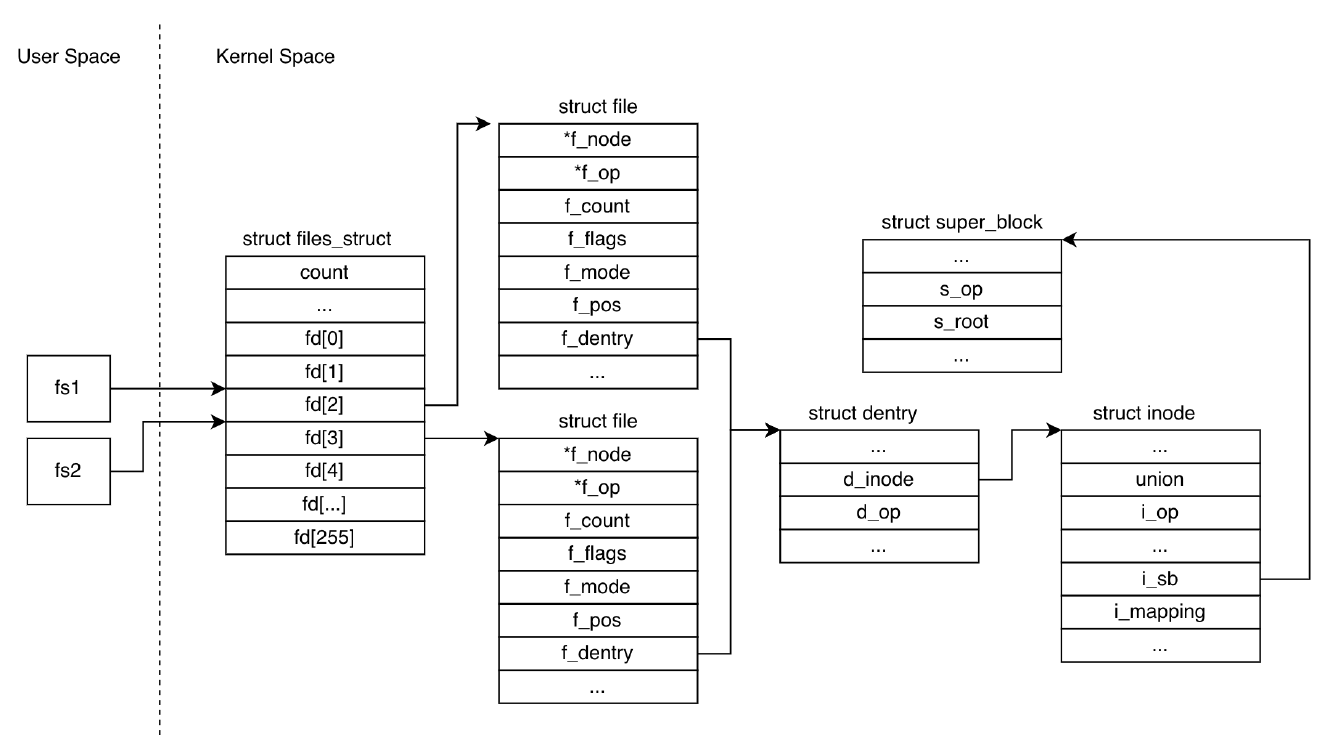
\includegraphics[scale=0.45]{p2_schema}
	\caption{Схема связи структур}
\end{figure}


\section*{Программа 3}

В данной программе открывается один и тот же файл два раза с использованием библиотечной функции fopen(). Для этого объявляются два файловых дескриптора типа FILE. В цикле записываются в файл буквы латинского алфавита, поочередно передавая функции fprintf() то первый дескриптор, то – второй.

\pagebreak

\subsection*{Однопоточный вариант}

\begin{lstlisting}[caption=Однопоточный вариант]
#include <stdio.h>
#include <sys/stat.h>
#include <unistd.h>

int main()
{
	FILE *fs1 = fopen("new_alphabet.txt", "a");
	FILE *fs2 = fopen("new_alphabet.txt", "a");
	char c = 'a';
	int flag = 0;
	while (c <= 'z')
		(flag = !flag) ? fprintf(fs1, "%c", c++) : fprintf(fs2, "%c", c++);
	struct stat filestat;
	fstat(fs1->_fileno, &filestat);
	printf("inode=%lu, size=%ld\n", filestat.st_ino, filestat.st_size);
	fclose(fs1);
	
	fstat(fs2->_fileno, &filestat);
	printf("inode=%lu, size=%ld\n", filestat.st_ino, filestat.st_size);
	fclose(fs2);
	
	stat("new_alphabet.txt", &filestat);
	printf("inode=%lu, size=%ld\n", filestat.st_ino, filestat.st_size);
	return 0;
}
\end{lstlisting}

Результат работы однопоточного варианта программы представлен на рисунках \ref{p3_one}, \ref{p3_one_stat}.

\begin{figure}[ht!]
	\centering
	
\includegraphics[scale=1]{p3_one}
	\caption{Результат работы однопоточной программы}
	\label{p3_one}
\end{figure}

\begin{figure}[ht!]
	\centering
	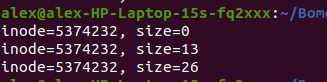
\includegraphics[scale=1]{p3_one_stat}
	\caption{Результат работы однопоточной программы}
	\label{p3_one_stat}
\end{figure}

\subsection*{Многопоточный вариант}

\begin{lstlisting}[caption=Многопоточный вариант]
#include <stdio.h>
#include <pthread.h>
#include <sys/stat.h>
#include <unistd.h>

void *thread(void *args)
{
	int shift = *(int *) args;
	FILE *fs = fopen("new_alphabet.txt", "a");
	char c = 'a' + shift;
	while (c <= 'z')
	{
		fprintf(fs, "%c", c);
		c += 2;
	}
	struct stat filestat;
	fstat(fs->_fileno, &filestat);
	printf("shift=%d, inode=%lu, size=%ld\n", shift, filestat.st_ino, filestat.st_size);
	fclose(fs);
	stat("new_alphabet.txt", &filestat);
	printf("shift=%d, inode=%lu, size=%ld\n", shift, filestat.st_ino, filestat.st_size);
	return NULL;
}

int main()
{
	pthread_t th1;
	pthread_t th2;
	int shift1 = 0;
	int shift2 = 1;
	pthread_create(&th1, NULL, thread, &shift1);
	pthread_create(&th2, NULL, thread, &shift2);
	pthread_join(th1, NULL);
	pthread_join(th2, NULL);
	return 0;
}
\end{lstlisting}

Результат работы многопоточного варианта программы представлен на рисунках \ref{p3_two}, \ref{p3_two_stat}.

\begin{figure}[ht!]
	\centering
	
\includegraphics[scale=1]{p3_two}
	\caption{Результат работы многопоточной программы}
	\label{p3_two}
\end{figure}

\begin{figure}[ht!]
	\centering
	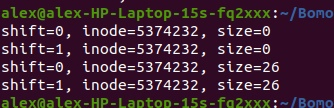
\includegraphics[scale=1]{p3_two_stat}
	\caption{Результат работы многопоточной программы}
	\label{p3_two_stat}
\end{figure}

\section*{Анализ результата}

Вызов функции fprintf с экземпляром структуры \_IO\_FILE приводит к тому, что соответствующий этому экземпляру буфер начинает заполняться, а данные на экран не выводятся. Так происходит, пока буфер не будет заполнен, не будет вызвана функция fflush для принудительного сброса содержимого буфера или не файл не будет закрыт. В данном случае печать происходит при закрытии файла, это видно из информации приведённой в структуре stat. Размер файла до закрытия равен 0, а после 13.

\begin{figure}[ht!]
	\centering
	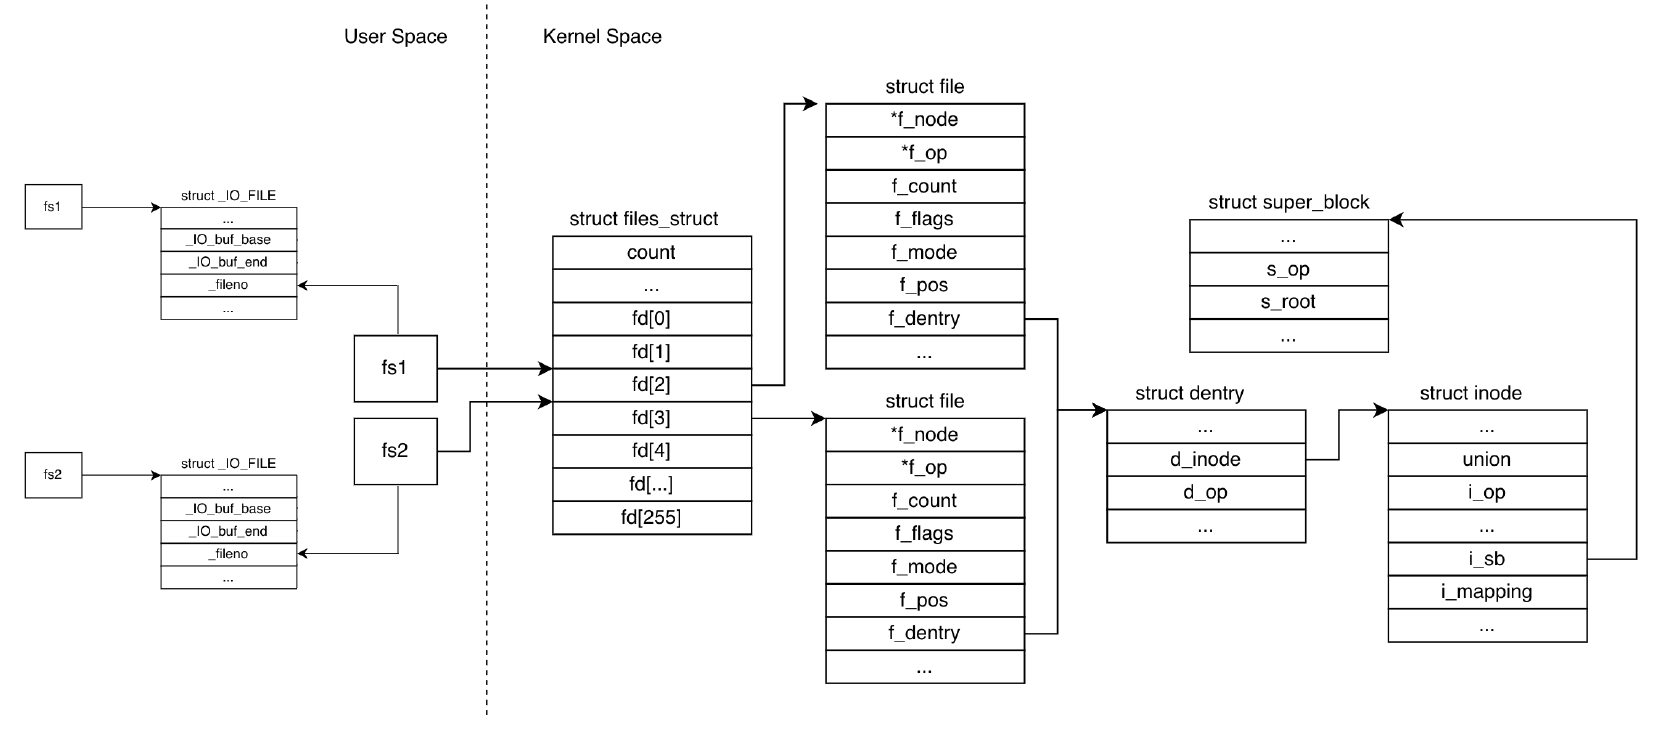
\includegraphics[scale=0.4]{p3_schema}
	\caption{Схема связи структур}
\end{figure}